%------------------------------- CHAPTER NAME --------------------------------
\chapter{High lift devices effects}
In the preliminary design of the wing a large number of requirements have to be fulfilled as exemplified in table~\ref{table:WingRequirements}; but, as many of them are in conflict, it is hardly ever possible to check them all, so that a compromise has to be found.

\begin{table}[!h]
\makebox[\linewidth]{
\begin{tabular}{l}
\toprule
\textbf{Wing design requirements} \\
\midrule
Low drag \\
High lift \\
Satisfactory maximum lift coefficient \\
Satisfactory stall quality \\
High value of the critical Mach number \\
Low weight \\
Ensure satisfactory performance in all flight phases \\
\bottomrule
\end{tabular}
}
\caption{Some wing design requirements}
\label{table:WingRequirements}
\end{table}

\noindent
With respect of the last shown requirement, the wing is usually equipped with high-lift devices, which change it's shape, in order to make it performant both in cruise both in take-off and landing phases. In fact, as can be seen from table~\ref{table:cruiseTOLand}, these phases show conflicting objectives which can only be mediated through the introduction of these devices.

\begin{table}[!h]
\makebox[\linewidth]{
\begin{minipage}{6cm}
\leftline{	
\begin{tabular}{l}
\toprule
\textbf{Cruise requirements} \\
\midrule
Small wing surface and high wing \\
loading $W/\!S$ \\ [0.1 cm] 
Small camber \\ [0.1 cm]
Low drag \\ [0.1 cm]
High speed \\ [0.1 cm]
Lift generated using low c\textsubscript{L} \\ 
\bottomrule
\end{tabular}
}
\end{minipage}
\hspace{2.5cm}
\begin{minipage}{6cm}
\rightline{
\begin{tabular}{l}
\toprule
\textbf{Take-Off and Landing requirements} \\
\midrule
Big wing surface, or high c\textsubscript{Lmax}, in order \\
to have an high equivalent wing loading \\
$m=W/(\!S\cdot c_{Lmax})$ \\ [0.2 cm]
High drag value in landing \\ [0.2 cm]
Lift generated using high c\textsubscript{L} due to the \\
low speed \\ 
\bottomrule
\end{tabular}
}
\end{minipage}
}
\caption{Comparison between cruise and take-off/landing design requirements}
\label{table:cruiseTOLand}
\end{table}

%-------------------------- THEORETICAL BACKGROUND ---------------------------
\section{Theoretical background}
In this paragraph, a general overview of the different type of high-lift devices is provided as well as the semi-empirical steps used to predict their effects on aerodynamic perofmance of the wing.

\bigskip
\noindent
The disigner may choose from a large collection of feasible high-lift systems, although in the case of a specific project this freedom will be limited, since incremental drag, mechanical complexity, development and maintenance costs and structural weight are all factors to be considered~\cite{torenbeek1982synthesis}.

\bigskip
\noindent
All high-lift devices can be divided in two main groups of which only the first one will be analyzed in this discussion:

\begin{itemize}
\item Systems for passive lift increase, such as \emph{leading-edge devices} or \emph{trailing-edge devices}, which modify the wing shape.
\item Systems for active lift increase, such as \emph{blown flaps} or \emph{jet flaps}, which acts directly on the flow in order to control it.
\end{itemize}

\noindent
Genrally speaking, \emph{trailing-edge devices} are used to increase the wing maximum lift coefficient, while \emph{leading-edge devices} are used to increase the stalling angle of attack. 

A more in depth analysis shows that \emph{trailing-edge devices} increase the camber and improve the flow at the trailing edge, but tend to promote leading edge stall on thin sections and may cause a reduction in the stalling angle of attack; on the other hand \emph{leading-edge devices} postpone or eliminate leading edge stall, but  they have little effects on the airfoil camber as a whole, although locally the camber is increased~\cite{torenbeek1982synthesis}.

\bigskip
\noindent
About \emph{trailing-edge devices}, their effects can be resumed in:

\begin{itemize}
\item Higher c\textsubscript{L} at a given angle of attack and higher c\textsubscript{Lmax}
\item Lower stalling angle of attack
\item Lower zero-lift angle due to increasing camber
\end{itemize}

\noindent
while \emph{leading-edge devices} provide the followings:
\begin{itemize}
\item Extension of the linear trait of the lift curve with an increase of the maximum angle of attack and of the c\textsubscript{Lmax}
\item Higher zero-lift angle due to translation of the lift curve on the right caused by leading edge deflection which reduce the actual angle of attack 
\item Higher slope of the linear trait of the lift curve, for those devices which extend airfoils chords with the effect of increase the wing surface and, with constant wing span, the aspect ratio
\end{itemize}

\begin{figure}
\centering
\begin{minipage}{.5\textwidth}
  \centering
  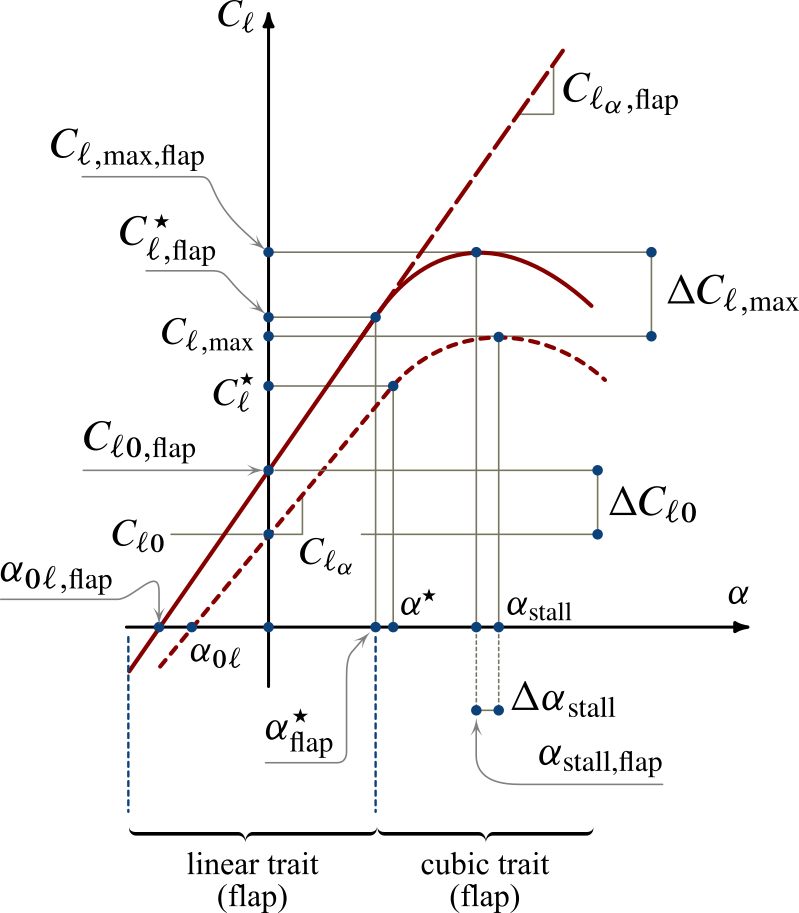
\includegraphics[width=.9\linewidth]{FlapEffects}
  \captionof{figure}{Trailing-edge devices effects}
  \label{fig:FlapEffects}
\end{minipage}%
\begin{minipage}{.5\textwidth}
  \centering
  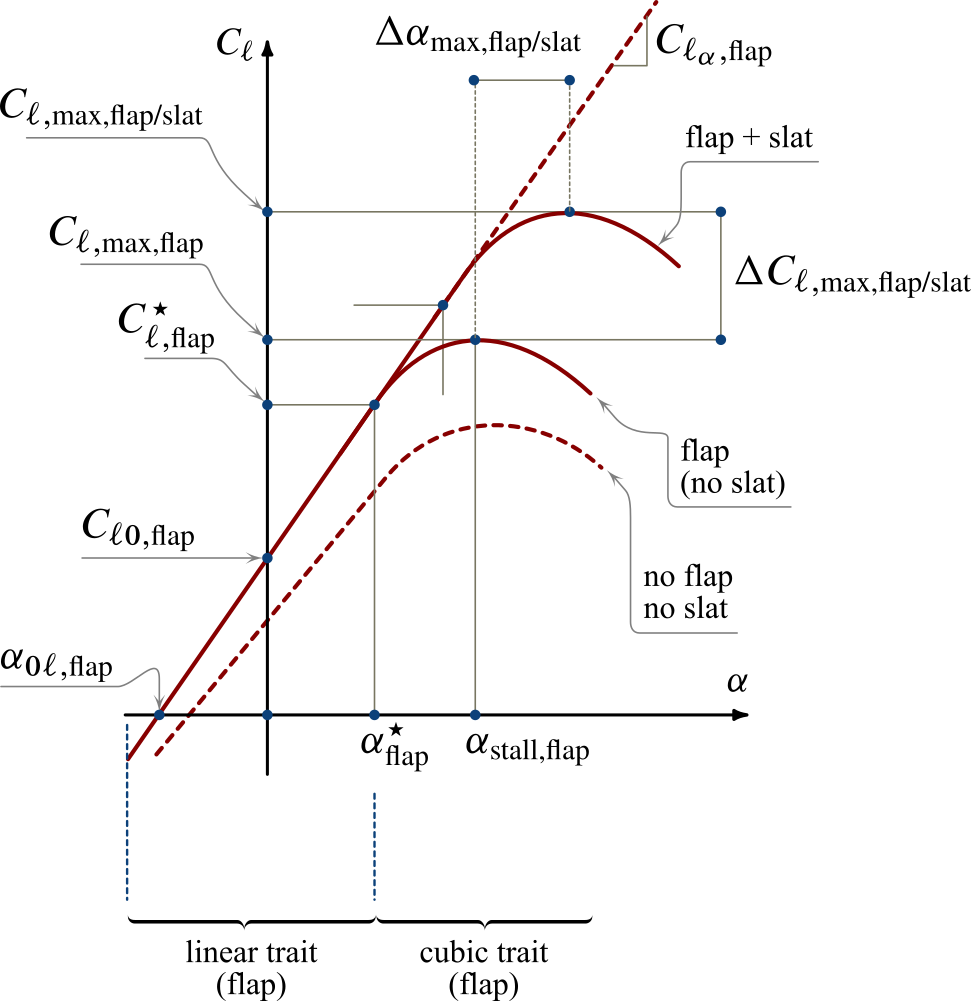
\includegraphics[width=\linewidth]{SlatEffects}
  \captionof{figure}{Leading-edge devices effects}
  \label{fig:SlatEffects}
\end{minipage}
\label{fig:FlapSlatEffects}
\end{figure}

\noindent
Among the variety of different devices, only the followings will be taken into account as they represents the most used ones.

\begin{itemize}
\item [\textbf{Plain flap}] This device is most used on small aircraft or ones equipped of a thin wing because it doesn’t support a complex mechanism of retraction. Typical deflections are about 20° for take-off and 60° for landing.
\item [\textbf{Single slotted flap}]  It can be seen as a plain flap with a gap between the two elements composing the airfoil. The single slotted flap has very little flap overlap with the fixed trailing edge and hence develops only little Fowler motion, that is the aft travel of the flap that increases the section chord. Its typical deflections are about 20° for take-off and 40° for landing.

The effects of a single slotted flap show an increment in all the aerodynamic coefficients, but it must be said that the increment in drag is lower than that for plain flaps. The slotted flap chord usually ranges from the 25\% up to the 30\% of the section chord. Moreover the slot influences boundary layer control, in fact it introduces a blowing that energizes the boundary layer delaying separation, so an increase in lift is generated.
\item[\textbf{Double slotted flap}] This device is superior to the previous type at large deflections, because separation of the flow over the flap is postponed by the more favourable pressure distribution. Its typical deflections are about 20° for take-off and 50° for landing; in particular, in order to avoid an increasing twisting moment due the deflection, this devices are usually combined with leading edge slats deflected of the same quantity. 
\item[\textbf{Triple slotted flap}] This device is used on several transport aircraft with very high wing loadings. In combination with leading edge devices, this system represents almost the ultimate achievement in passive high-lift technology, but its shape shows that complicated flap supports and controls are required. Its typical deflections are about 20° for take-off and 40° for landing.
\item[\textbf{Fowler flap}]  It is theoretically a single slotted flap that adds to the downward deflection also a backward motion that allows the increment of the effective chord and camber.

Due to the necessity of keeping the rear part of the wing section extended out the main element its implementation system is usually more complicated than the single slotted flaps but its weight and costs are largely justified by its high lift effectiveness. Its typical deflection are about 40° for landing and 15° for take-off, smaller than other types because the chord extension provides a bigger lift increment due to the bigger wing surface; this also reduces the drag in take-off wth benefit an the required field length.
\item[\textbf{Slat}]  It's the most efficient leading edge device; thanks to combined deflection and forward motion, it acts in order to increase airfoil camber, and so the maximum lift coefficient, as well as increase the airfoil chord with the result of a bigger surface which provides a bigger aspect ratio with the effect of increase the lift curve slope of the linear trait. Furthermore, thanks to the slot which provides a boundary layer energization, it also increases the stalling angle of attack.
\item[\textbf{Kruger flap}]  It acts in the same way as the slat, but it is thinner and more suitable for installation on thin wings. Krueger flaps are very common because of their simple architecture.
\item[\textbf{Plain leading edge flap}] Is less effective than slat since it has no slot, it is mechanically simple and rigid and particularly suitable for thin airfoil sections. The leading edge can be hinged in order to move it backward (droop nose) or it has a mechanism inside that changes the curvature of the nose (variable camber flap).
\item[\textbf{Leading edge fixed slot}] It has a fixed slot at the leading edge that, at high angle of attack, allows the airflow to pass through energizing the boundary layer; this helps to increase the stalling angle of attack. During the criuse phase, in which the angle of attack is small, the gap is usually seald.
\end{itemize}

\begin{figure}[!t]
  \centering
  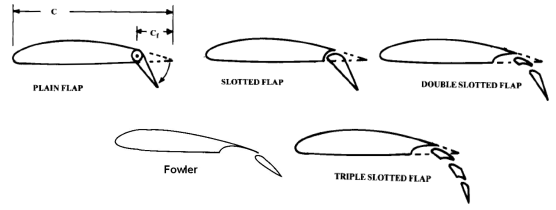
\includegraphics[width=\linewidth]{Flap}
  \caption{Analyzed trailing edge devices types}
  \label{fig:FlapTypes}
\end{figure}

\begin{figure}[!t]
  \centering
  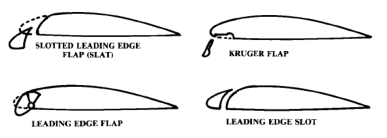
\includegraphics[width=0.7\linewidth]{Slat}
  \caption{Analyzed leading edge devices types}
  \label{fig:SlatTypes}
\end{figure}
%%-------------------------------------------------------------INSERT FLAP/SLAT TYPE FIGURE-----------------------------------------------------------------------------

\noindent
In order to predict, from the preliminary design phase, the aerodynamic characteristics of the high-lift devices, some useful semi-empirical methods are available; in this particular case the followings formulas and charts are taken from~\cite{torenbeek1982synthesis} and~\cite{sforza2014commercial}.

\bigskip
\noindent
The guideline that will be followed provides to analyze separately the trailing edge and the leading edge devices effects; moreover it will start by evaluating the changes in aerodynamic characteristics of airfoils for then extends these to entire wing.

From figures~\ref{fig:FlapEffects} and~\ref{fig:SlatEffects}, it's possible to understand that the main changes introduced by trailing edge, or leading edge, devices are related to the evaluation of four quantities:

\begin{itemize}
\item $\Delta c_{l0}$
\item $\Delta c_{l\text{max}}$
\item $c_{l\alpha, \text{flap}}$
\item $\Delta\alpha_{\text{stall}}$
\end{itemize}

%------------------------- DeltaCl0 & DeltaCL0 subsection---------------------------
\subsection{$\Delta c_{l0}$ and  $\Delta c_{L0}$ calculation}
An empirical method for predicting airfoil lift increments at zero angle of attack for high-lift systems $\left(\Delta c_{l0}\right)$ comes from the Glauert’s linearized theory for thin airfoils with flaps. A result obtained from this theory for the lift due to flap deflection is the following.

\begin{equation}
\alpha_\delta=1-\frac{\theta_f-\sin(\theta_f)}{\pi}
\label{eqn:AlphaDelta}
\end{equation}

\noindent
where

\begin{equation}
\theta_f=\cos^{-1}\left(2\ \frac{c_f}{c}-1\right)
\label{eqn:ThetaF}
\end{equation}

\noindent
Known this value, it's possible to evaluate the theoretical $\Delta c_{l0}$ which can be calculated as proposed in (\ref{eqn:DeltaCl0}).

\begin{equation}
\Delta c_{l0}=\alpha_\delta\ c_{l\alpha}\ \delta_f
\label{eqn:DeltaCl0}
\end{equation}

\noindent
with $c_{l\alpha}$ equals to the linear slope of the llift curve of the airfoil, and $\delta_{f}$ the flap angular deflection.

For large flap deflections and for the separation at large flap angles due to viscosity, linear theory is in error when compared with exact one, for this reason we assume the effectiveness factor $\eta_\delta$, so the formulation becomes the following.

\begin{equation}
\Delta c_{l0}=\alpha_\delta\ c_{l\alpha}\ \delta_f\ \eta_\delta
\label{eqn:DeltaCl0EtaDelta}
\end{equation}

\noindent
where $\eta_\delta$ can be evaluated from the charts provided in figures~\ref{fig:EtaDeltaPlain} and~\ref{fig:EtaDelta}.

\begin{figure}[!t]
  \centering
  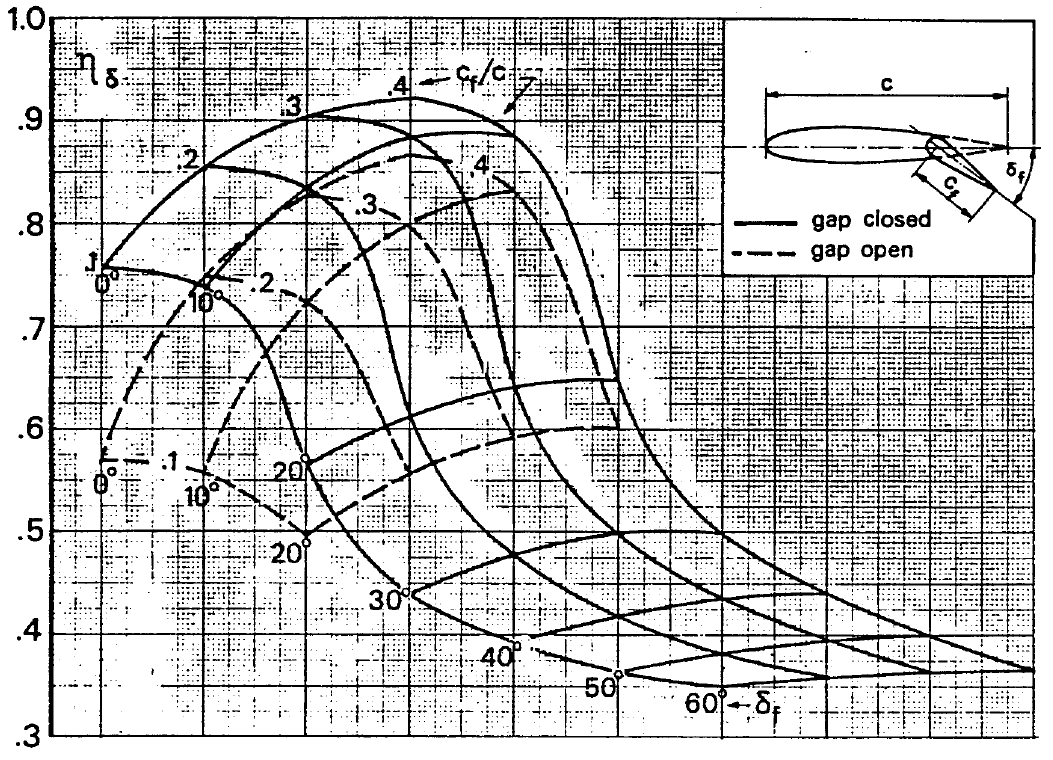
\includegraphics[width=0.65\linewidth]{Eta_Delta_Plain}
  \caption{$\eta_\delta$ for plain flap}
  \label{fig:EtaDeltaPlain}
\end{figure}

\begin{figure}[!b]
  \centering
  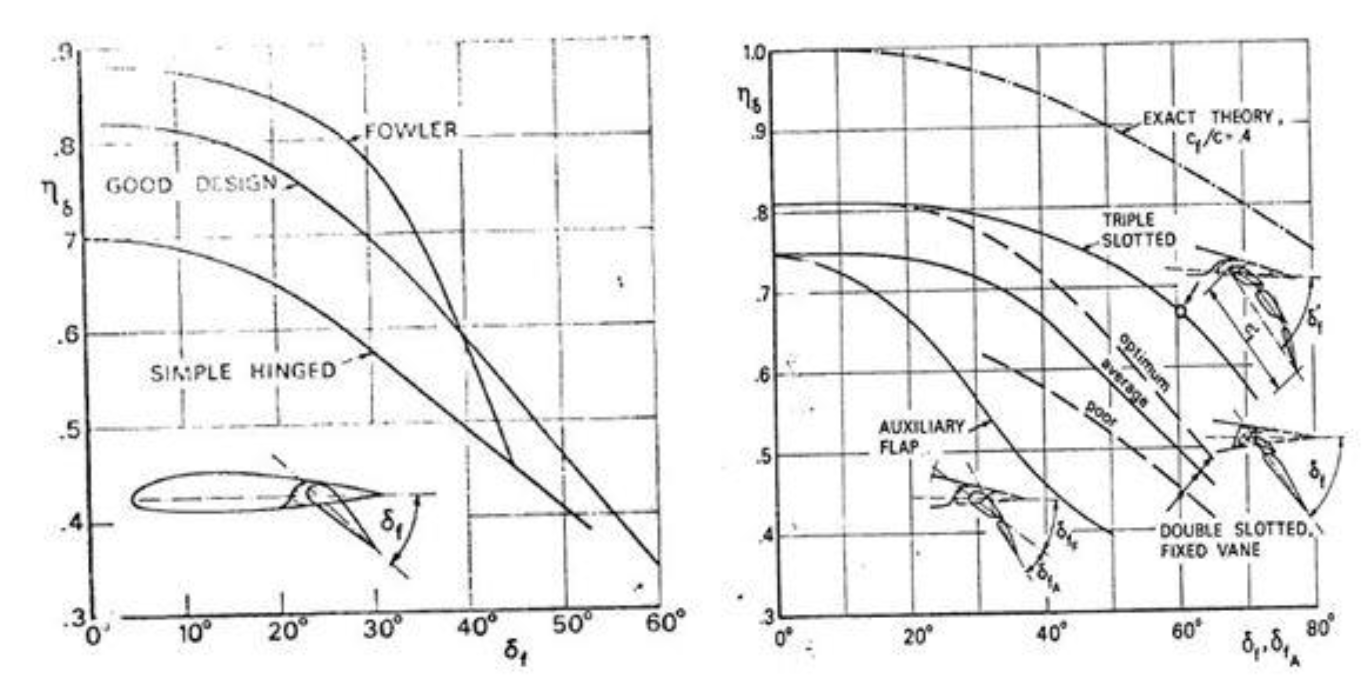
\includegraphics[width=\linewidth, angle=359]{Eta_Delta}
  \caption{$\eta_\delta$ for other type of flaps}
  \label{fig:EtaDelta}
\end{figure}

\noindent
In case of flaps which extend the airfoil chord, this effects also contributes to the lift increase and can be taken into account by referring the section lift to the extended chord and then converting the result to the original chord. As a results of this, the section lift coefficient can be evaluated as shown in (\ref{eqn:clExtendedChord}).

\begin{equation}
c_{l}=\left(c_{l0}'+\Delta c_{l0}'\right)\ \frac{c'}{c}
\label{eqn:clExtendedChord}
\end{equation}

\noindent
where the variables with superscript are referred to the extended chord. Assuming that for the basic section $c_{l0}'=c_{l0}$, it's possible to derive the $\Delta c_{l0}$ as folllows.

\begin{equation}
\Delta c_{l0}=\Delta c_{l0}'\ \frac{c'}{c}+c_{l0}\left(\frac{c'}{c}-1\right)
\label{eqn:Deltacl0Final}
\end{equation}

\noindent
in which $c_{l0}$ is known, $\Delta c_{l0}'$ is calculated as in (\ref{eqn:DeltaCl0EtaDelta}) and $\frac{c'}{c}$ is equal to the following expression.

\begin{equation}
\frac{c'}{c}=1+\frac{\Delta c}{c_f}\ \frac{c_f}{c}
\label{eqn:c'/c}
\end{equation}

\noindent
where $\frac{\Delta c}{c_f}$ can be derived from the charts of figure~\ref{fig:DeltaCCf}.

\begin{figure}[!t]
  \centering
  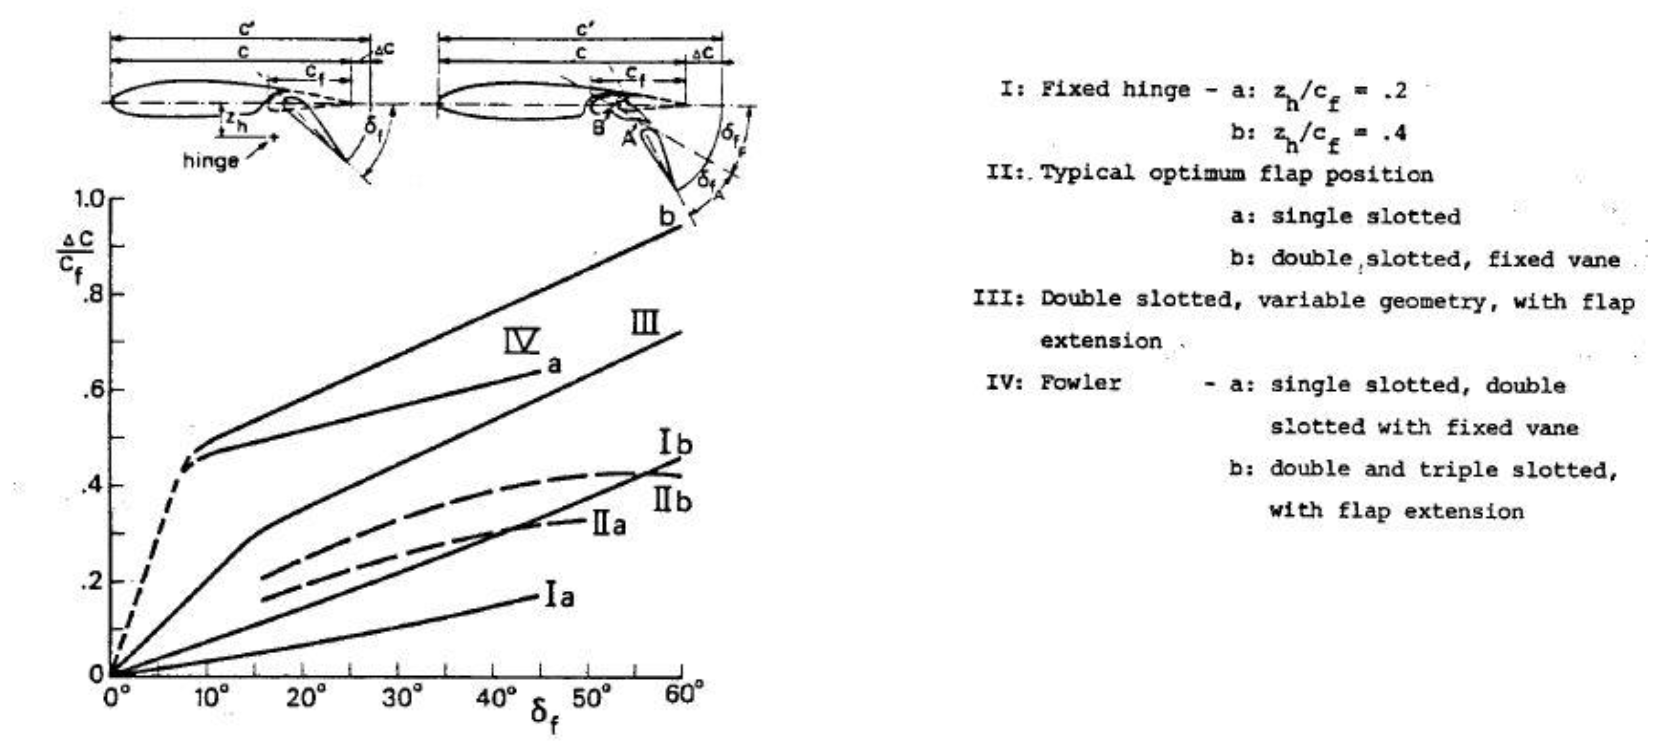
\includegraphics[width=\linewidth, angle=0.5]{DeltaC_Cf}
  \caption{$\frac{\Delta c}{c_f}$ for different type of flaps as function of flap deflection}
  \label{fig:DeltaCCf}
\end{figure}

\noindent
The $\Delta c_{l0}$ so calculated has now to be extended to the entire wing; this can be through the following forumla.

\begin{equation}
\Delta c_{L0}=\Delta c_{l0}\ \left(\frac{c_{L\alpha}}{c_{l\alpha}}\right)\ \left[\frac{\left(\alpha_\delta\right)_{c_{L}}}{\left(\alpha_\delta\right)_{c_{l}}}\right]\ K_b
\label{eqn:c'/c}
\end{equation}

\noindent
where $c_{L\alpha}$ and $c_{l\alpha}$ are respectively the lift curve slopes of the wing and the airfoil, $\left[\frac{\left(\alpha_\delta\right)_{c_{L}}}{\left(\alpha_\delta\right)_{c_{l}}}\right]=K_c$ is the ratio of the three-dimensional flap effectiveness parameter to the two dimensional flap effectiveness one, which can be derived from the figure~\ref{fig:Kc}, and $K_b$ is a flap span effectiveness factor, which is function of the flap span-wise extension, that can be  read from~\ref{fig:Kb}.

\begin{figure}[!b]
  \centering
  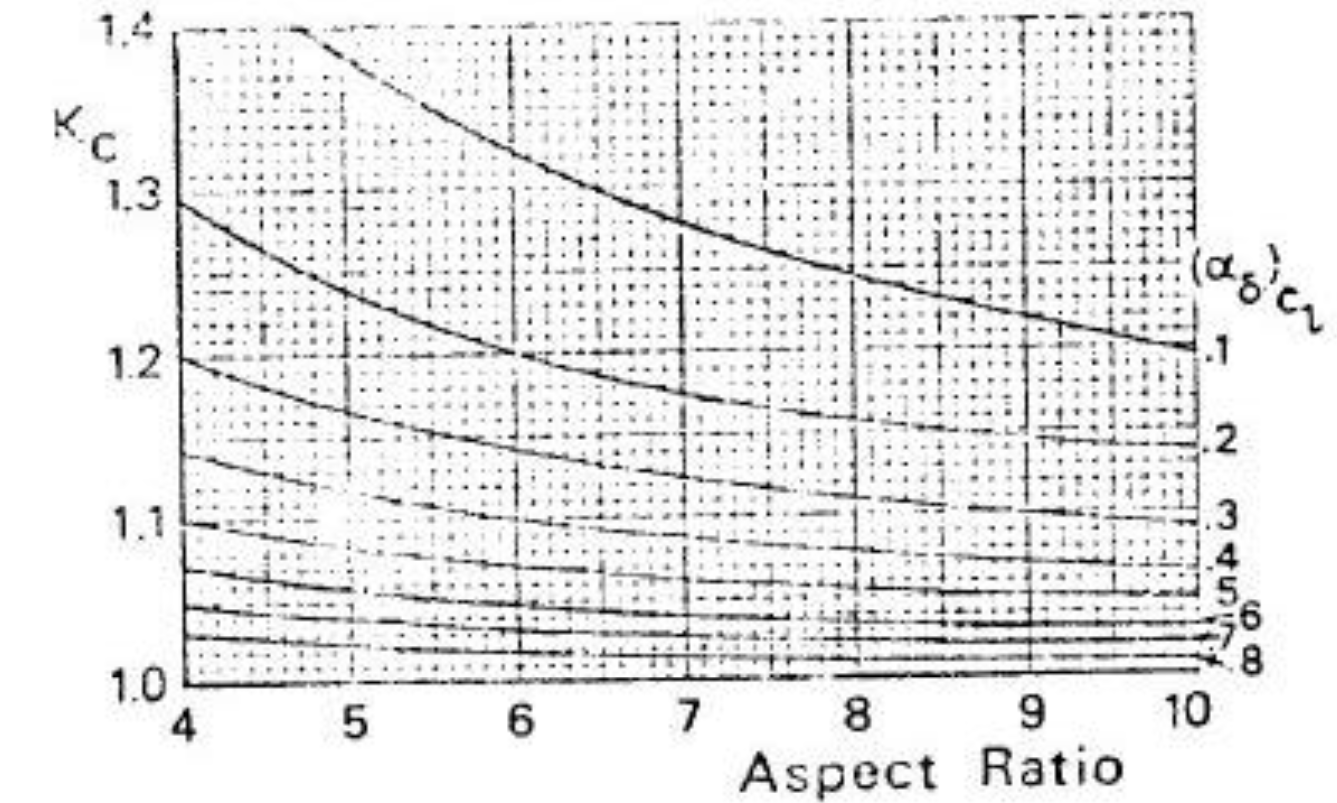
\includegraphics[width=0.7\linewidth, angle=359]{Kc}
  \caption{$K_c$ for different $\left(\alpha_\delta\right)_{c_{L}}$ as function of wing aspect ratio}
  \label{fig:Kc}
\end{figure}

\begin{figure}[!t]
  \centering
  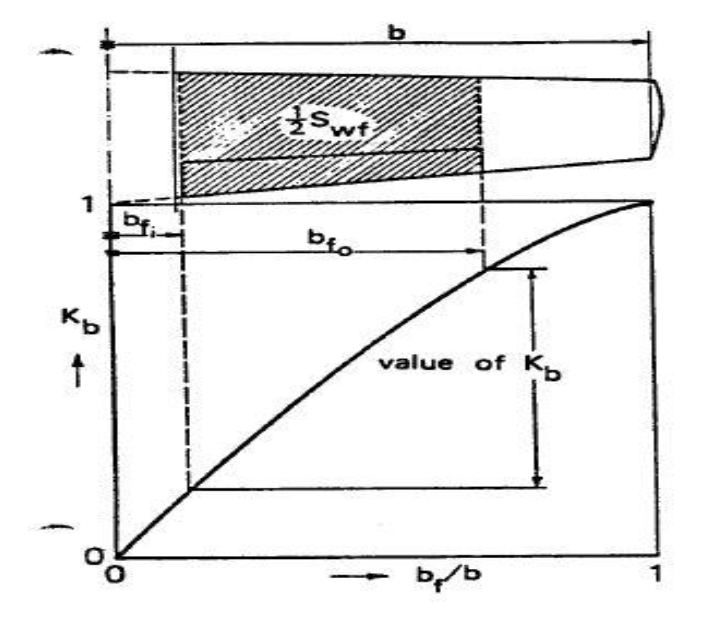
\includegraphics[width=0.5\linewidth, angle=359]{Kb}
  \caption{$K_b$ as function of flap span to wing span ratio ($\frac{b_f}{b}$)}
  \label{fig:Kb}
\end{figure}

%------------------------- DeltaClmax & DeltaCLmax subsection---------------------------
\subsection{$\Delta c_{l\text{max}}$ and  $\Delta c_{L\text{max}}$ calculation for flaps and slats}
%--------------------------- Cl_alpha & CL_alpha subsection-------------------------------
\subsection{$c_{l\alpha, \text{flap}}$ and  $c_{L\alpha, \text{flap}}$ calculation}
%------------------------------ DeltaAlphaMax subsection-----------------------------------
\subsection{$\Delta\alpha_{\text{stall}}$ calculation for flaps and slats}
%---------------------------  DeltaCD & DeltaCM subsection--------------------------------
\subsection{Further effects calculations}


%------------------------- JAVA CLASS ARCHITECTURE ---------------------------
\section{Java class architecture}
%----------------------- CASE STUDY : ATR72 AND B747 -------------------------
\section{Case study: ATR-72 and B747-100B}
